\chapter{自旋交换相互作用体系少体精确解}\label{chap:kondo}

受到最近在超冷碱土金属平台中模拟近藤物理的实验以及理论进展的启发,采用严格对角化的数值方法,我们精确地研究了一维谐振子势场下一个局域磁性杂质与一个以及两个巡游费米子在自旋交换相互作用支配下的1+1以及1+2少体体系的能谱结构。在1+1少体体系中,我们发现对应于不同的铁磁、反铁磁耦合,少体精确解中的attractive branch与repulsive branch具有不同的磁性结构。对于1+2少体体系,在反铁磁耦合下的attractive branch中我们发现了类似于多体物理中的近藤屏蔽效应。进一步地,我们在反铁磁耦合体系中发现了一系列铁磁repulsive branch,它们与其他的attractive branch正交,并且其波函数拥有良好的自旋电荷分离的特点。最后,我们还简单探讨了实际体系中经常带有的接触相互作用带来的影响以及向多体体系的推广。我们的结果尝试从少体的角度发觉带有自旋交换相互作用影响的体系所独有的内禀物理特性,并期待可以在未来的超冷原子实验中得到实现与探索。

在~\ref{sec:spex-intro}~节中,我们介绍这一工作的背景和动机。在~\ref{sec:spex-model}~节中,我们介绍考虑的少体模型以及求解的数值方法。在~\ref{sec:spex-result}~节中,我们讨论得到结果并揭示其物理图像。在~\ref{sec:spex-summary}~节中,我们总结我们的结果并做后续研究的展望。

\section{引言}\label{sec:spex-intro}
在本论文的第一章里面~\ref{sec:spin-exchange}~中我们系统的介绍了自旋交换相互作用在超冷碱土金属原子中的研究进展。总体来讲,利用最外层2个电子的中性原子的基态${}^1S_0$与激发态${}^3P_0$来组成两轨道体系,整个原子的核自旋作为每个粒子的自旋自由度。不同轨道之间的自旋交换相互作用由实验所证实,其中裸的铁磁交换相互作用由${}^{173}$Yb\cite{scazza2014observation,cappellini2014direct,pagano2015strongly,hofer2015observation}与${}^{87}$Sr\cite{zhang2014spectroscopic}原子实现,而裸的反铁磁交换相互作用由${}^{171}$Yb\cite{ono2019antiferromagnetic}原子实现。通过使用束缚诱导共振技术,我们可以方便地低维度下体系的自旋交换相互作用的强度。这种调节已由理论和实验所证实\cite{zhang2016kondo,cheng2017enhancing,zhang2018control,ji2018confinement,zhang2020tight,zhang2020controlling,riegger2018localized}。进一步地,在近藤物理模拟中起关键作用的局域磁性杂质可以借由“魔法”频率光晶格来实现,其原理在于选取合适频率的激光形成光晶格,这种特殊的光晶格利用不同原子态的交流极化率来有选择性的使${}^3P_0$态的原子被束缚住,而${}^1S_0$态的原子则可以自由运动\cite{riegger2018localized,barber2008optical}。上述实验技术与理论计算的进展使得冷原子平台模拟多体近藤物理不再遥远。

不止于此,基于目前的研究进展,我们发现已经可以将目光聚集在少体体系。不同于多体体系,少体体系其独有的理论精确解为理解其中的物理提供坚实的基础。其中简洁的物理图像不仅为少体体系独有,而且为理解与表征多体体系提供丰富的线索。在本文的~\ref{sec:fewbody}~里面我们讨论了相关的背景,{\color{red} 待补充 }


综上,我们发现带有自旋交换相互作用的少体体系亟需系统的研究。因此在这一章节中,我们采用严格对角化的数值方法,系统地求解了1维简谐势场下带有自旋交换相互作用的1+N少体体系:
\begin{equation}\label{eq:sp-ex}
    \adddotsbeforeeqnnum%
    \hat{U}_{ex} = J\cdot\sum_{j=1}^{N}\hat{\Vector{S}}_j\cdot\hat{\Vector{S}}\cdot \delta(x_j)
\end{equation}
其中前面的1为局域带自旋1/2的磁性杂质(自旋算符为$\hat{\Vector{S}}$),位于原点处。后部面的N代表带自旋1/2的巡游费米子(自旋算符为$\hat{\Vector{S}}_j$),在本文中我们研究$N=1,2$。我们考虑杂质与费米子之间各向同性的铁磁与反铁磁海森堡耦合,其耦合强度可以调节。早在1980年代,描述一维连续空间里的费米子与局域自旋杂质体系的多体近藤模型就可用贝特假设的办法严格求解\cite{andrei1983solution},不过其前提在于假设费米子的色散关系为线性($\epsilon_k\propto k$),并带有可重整化的cut off。在这个假设下得到的结果,只有当费米海附近的费米子被自旋杂质散射时才成立,这对应若耦合极限附近。作为对比,在我们这一章节讨论当中,我们求解从弱到强整个相互作用区间的少体能谱与波函数,旨在得到系统的少体物理结果,为多体体系的研究提供启发。


最终,我们的结果总结如下:在自旋交换相互作用支配下的少体体系,展示了不同于纯接触相互作用少体体系的新奇特性。attractive 与 repulsive branch 的磁性结构由自旋交换的铁磁$J<0$与反铁磁$J>0$所决定。重要地,对于1+2的少体体系,我们发现对于反铁磁耦合,基态的attractive branch展现出一种屏蔽效应,而铁磁耦合的attractive branck则没有这种屏蔽。进一步,我们在反铁磁耦合这边发现了一系列的铁磁upper branch激发态,这些特殊的铁磁branch与其它的attractive branch没有发生level avoid crossing,其波函数具有很好的自旋电荷分离的特性。这些新奇的现象都来自于自旋交换相互作用,相应的branch也很容易在碱土金属原子实验中去探测,最后我们还考虑了实际体系经常伴有的纯接触相互作用的影响,以及简单的从少体物理特性到多体物理特性的推广。

\section{模型与计算}\label{sec:spex-model}
我们首先详尽的给出考虑的1+1与1+2少体体系的哈密顿量,并结合具体的物理意义给出变分波函数,最终推导出用于数值求解的矩阵方程。
\subsection{1+N体系哈密顿量}
我们的1+N少体体系处于一维简谐势场中,一个局域的自旋杂质被固定在原点$x=0$处,仅有自旋自由度,空间自由度被冻结。N个巡游费米子在一维连续空间运动,坐标表象下其位置为$x_j,j=1,...,N$。巡游费米子与局域自旋杂质之间存在自旋交换相互作用,整个体系的哈密顿量为(我们在本章中取$\hbar=1$):
\begin{equation}\label{eq:spex-hamiltonian}
\adddotsbeforeeqnnum%
    \begin{split}
       	\hat{H}  &= \hat{H}_0 + \hat{U}_{ex}\\
		\hat{H}_0 &= \sum_{j=1}^{N} \left( -\frac{1}{2M} \frac{\partial^2}{\partial x_{j}^2}   +\frac{M\omega^2}{2}x_{j}^2 \right); \\
		\hat{U}_{ex} &= 2J\cdot\sum_{j=1}^N\delta(x_j){\hat{\Vector{S}}}_j\cdot {\hat{\Vector{S}}}.
    \end{split}
\end{equation}
其中$M$为巡游费米子的质量,$\omega$为谐振子的特征频率,$\hat{\Vector{S}}=(\hat{S}_{x},\hat{S}_{y},\hat{S}_{z})$与$\hat{\Vector{S}}_j=(\hat{S}_{jx},\hat{S}_{jy},\hat{S}_{jz})$分别代表杂质与费米子自旋算符。展开为产生湮灭场算符为:
\begin{equation}\label{eq:spex-field}
\adddotsbeforeeqnnum%
    \begin{split}
		\hat{S}_{jx} &= \frac{1}{2}(\hat{\psi}_{\uparrow}^{\dag}(x_j)\hat{\psi}_{\downarrow}(x_j)+\hat{\psi}_{\downarrow}^{\dag}(x_j)\hat{\psi}_{\uparrow}(x_j));\\
		\hat{S}_{jy} &= \frac{-i}{2}(\hat{\psi}_{\uparrow}^{\dag}(x_j)\hat{\psi}_{\downarrow}(x_j)-\hat{\psi}_{\downarrow}^{\dag}(x_j)\hat{\psi}_{\uparrow}(x_j));\\
		\hat{S}_{jz} &= \frac{1}{2}(\hat{\psi}_{\uparrow}^{\dag}(x_j)\hat{\psi}_{\uparrow}(x_j)-\hat{\psi}_{\downarrow}^{\dag}(x_j)\hat{\psi}_{\downarrow}(x_j)).
    \end{split}
\end{equation}
其中$\hat{\psi}_{\sigma}^{\dag}(x)$为在x处产生一个自旋为$\sigma(\uparrow,\downarrow)$的费米子产生算符。在谐振子基矢下其展开式为:
\begin{equation}
\adddotsbeforeeqnnum%
	\hat{\psi}_{\sigma}^{\dag}(x)=\sum_m \hat{C}_{m\sigma}^{\dag} \phi_m(x).
\end{equation}
其中$\hat{C}_{m\sigma}^\dagger$是产生一个处于第$m$个简谐振子能级的带有自旋$\sigma$费米子的产生算符,该能级的本征波函数在坐标表象下记为$\hat{\phi}_m(x)$,本征能量为$E_m = (m+\frac{1}{2})\omega$。在这套完备的谐振子基矢下系统的哈密顿量(\ref{eq:spex-hamiltonian})可以重新写为二次量子化形式:
\begin{equation}
	\begin{split}
		\hat{H} &= \sum_{m\sigma}E_m \hat{C}_{m\sigma}^\dagger \hat{C}_{m\sigma} + \sum_{m,n} \hat{V}_{mn} ( \hat{C}_{m\uparrow}^\dagger  \hat{C}_{n\downarrow} \hat{S}_- + h.c. \\
     	& +   (\hat{C}_{m\uparrow}^\dagger  \hat{C}_{n\uparrow}-\hat{C}_{m\downarrow}^\dagger  \hat{C}_{n\downarrow}) \hat{S}_{z} ), \label{eq:H2}\\
\end{split}
\end{equation}
其中$V_{mn} = J\phi_m(0)\phi_n(0)$是自旋交换相互作用$\hat{V}_{ex}$导致的$m,n$本征态之间跃迁的矩阵元。我们记$|\Uparrow\rangle$ 与$|\Downarrow\rangle$为局域杂质的自旋态,因此我们有$S_+=|\Uparrow\rangle\langle \Downarrow|$,$S_-=|\Downarrow\rangle\langle \Uparrow|$,而$S_z=(|\Uparrow\rangle\langle \Uparrow|-|\Downarrow\rangle\langle \Downarrow|)/2$。我们可以清楚得看到自旋交换过程是由(\ref{eq:H2})中括号里面的前两项实现的。

接下来我们给出用于具体求解少体能谱的计算公式。包括1+1与1+2自旋交换作用少体体系。

\subsection{一个杂质与一个费米子}
由于哈密顿量(\ref{eq:H2})依然具有自旋$SU(2)$旋转对称性。1+1少体体系按照一个杂质与一个费米子系统总的自旋$\hat{\Vector{S}}_{tot}$划分为自旋三重态通道($\hat{\Vector{S}}_{tot}=1$)与自旋单重态通道($\hat{\Vector{S}}_{tot}=0$)。每个独立的通道都是自旋算符的本征态。因此我们有每个通道的有效描述:
\begin{equation}
U_{s,t}(x_1)=\gamma_{s,t}\delta(x_1).
\end{equation}
其中单重态($singlet$)通道下费米子与杂质的有效耦合强度为$\gamma_s = \frac{-3J}{2}$,三重态($triplet$)通道下费米子与杂质的有效耦合强度为$\gamma_t = \frac{J}{2}$。

为了在同一个变分波函数中包含单重态通道与三重态通道的共同表达式,我们将波函数取在($S_{tot,z}=0$)的封闭子希尔伯特空间中:
\begin{equation}
	|\Psi\rangle_2=\sum_m \left( \phi_m^1 \hat{C}_{m\uparrow}^\dagger|0\rangle \Downarrow+ \phi_m^2 \hat{C}_{m\downarrow}^\dagger|0\rangle \Uparrow \right).
\end{equation}
其中$|0\rangle$是具有0个费米子的真空态。将波函数带入到薛定谔方程:
\begin{equation}
	\hat{H} |\Psi \rangle_2 = E |\Psi\rangle_2,
\end{equation}
我们得到如下的耦合方程组
\begin{equation}
    \begin{split}
      (E-E_m) \phi^1_m &= \sum_p (V_{mp}\phi^2_p-\frac{1}{2}V_{mp}\phi^1_p )\\
      (E-E_m) \phi^2_m &= \sum_p (V_{mp}\phi_p^1 -\frac{1}{2}V_{mp}\phi^2_p).
    \end{split}
\end{equation}
我们从中可以看到这组耦合方程有两类解,其中一类是:
\begin{equation}
    \phi^1_m=\phi^2_m \propto \frac{\phi_m(0)}{E-E_m},
\end{equation}
容易发现,这类解对应的是一个自旋三重态,其能量$E(=E_t)$满足自洽方程:
\begin{equation}
      \frac{1}{\gamma_t} =  \sum_m \frac{|\phi_m(0)|^2}{E_t-E_m}. \label{eq_t}
\end{equation}
而另一类解对应的是一个自旋单重态:
    \begin{equation}
      \phi^1_m = -\phi^2_m\propto \frac{\phi_m(0)}{E_s-E_m},
    \end{equation}
其能量$E(=E_s)$满足自洽方程:
	\begin{equation}
      \frac{1}{\gamma_s} =  \sum_m \frac{|\phi_m(0)|^2}{E_s-E_m}. \label{eq_s}
    \end{equation}
进一步地,两个自洽方程(\ref{eq_t},\ref{eq_s})可以统一为一个方程:
    \begin{equation}
        -\frac{2\sqrt{\pi}}{\kappa_{s,t}} = B(-\frac{\rho_{s,t}}{2},\frac{1}{2}) 
    \end{equation}
其中$\kappa_{s,t} \equiv \gamma_{s,t}\sqrt{M/\omega}$, $\rho_{s,t} \equiv E_{s,t}/\omega-1/2$,而$B(x,y)$是特殊函数中的贝塔函数。

\subsection{一个杂质与两个费米子}
有了1+1体系的求解,我们进一步考虑如果再增加一个自由费米子变成1+2体系,会出现如何有趣的物理呢?对于1个杂质和2个费米子的三体体系,系统总的自旋$\hat{\Vector{S}}_{tot}$可以为$\hat{\Vector{S}}_{tot}=1/2$或者$\hat{\Vector{S}}_{tot}=3/2$。同样地出于统一求解两种总自旋态的角度,我们仍然考虑$S_{tot,z}=1/2$的封闭子希尔伯特空间。其变分波函数可以写为:
\begin{equation}\label{eq:wv3}
    |\Psi\rangle_3 = \sum_{mn} \left( \phi^1_{mn} \hat{C}_{m\uparrow}^\dagger \hat{C}_{n\uparrow}^\dagger \left|0\right> |\Downarrow\rangle + \phi^2_{mn}  \hat{C}_{m\uparrow}^\dagger \hat{C}_{n\downarrow}^\dagger \left|0\right> |\Uparrow\rangle \right).
\end{equation}
其中,出于对2个费米子交换反对称的考虑,我们要求$\phi^1_{mn} = -\phi^1_{nm}$。将变分波函数带入薛定谔方程:
\begin{equation}
  \hat{H} |\Psi \rangle_3 = E |\Psi\rangle_3,
\end{equation}
我们得到变分参数满足的耦合方程组:
\begin{equation}
    \begin{split}
        &\phi^1_{mn} = \frac{1}{E-E_m-E_n} \cdot \frac{1}{2} \cdot  \sum_{p}-V_{mp}\phi^2_{np}+V_{np}\phi^2_{mp} +V_{np}\phi^1_{pm}- V_{mp}\phi^1_{pn} \\
        &\phi^2_{mn} = \frac{1}{E-E_m-E_n} \sum_p V_{np}\phi^1_{mp}-V_{np}\phi^1_{pm}+ \frac{1}{2} V_{mp}\phi^2_{pn}- \frac{1}{2}V_{np}\phi^2_{mp}.
    \end{split}\label{eq:eq_3b}
\end{equation} 
可以看到$\phi^1_{mn}$的交换反对称性依然成立。
仔细观察耦合方程(\ref{eq:eq_3b})的结构,我们发现可以进一步引入辅助变量$F^1_m,F^2_m,F^3_m$来减小体系求解的自由度数目,其背后的物理来源于在自旋交换相互作用是$s$波接触势,其中的一费米子和杂质形成二聚体(dimer)态:
    \begin{equation}
        \begin{split}
        &F^1_n \equiv \sum_p\phi_p(0)\phi^1_{np} \\
        &F^2_n \equiv \sum_p\phi_p(0)\phi^2_{np} \\
        &F^3_n \equiv -\sum_p\phi_p(0)\phi^2_{pn}\\
        \end{split} \label{F}
    \end{equation}
然后我们把方程(\ref{eq:eq_3b})左右两边同时乘以$\phi_m(0)$并对$m$求和可以得到一组新的$F^(i)_m$所满足的耦合方程。为了使得其物理意义更加明显,我们对引入的辅助变量$F^(i)_m$做线性叠加组合为$\tilde{F}^{(1)}_m$:
\begin{equation}
    \begin{split}
        &\tilde{F}^{(1)}_n =-\frac{3}{2}F_n^{(1)} +\frac{3}{4}F_n^{(2)}\\
        &\tilde{F}^{(2)}_n =\frac{1}{2}F_n^{(1)}+\frac{1}{4}F_n^{(2)} \\
        &\tilde{F}^{(3)}_n =\frac{1}{2}F_n^{(3)}.
    \end{split} \label{tF}
\end{equation}
经过这样的线性变换之后,变分波函数(\ref{eq:wv3})有了很直观的原子-二聚体分离的波函数:
 \begin{equation}
    \begin{split}
        |\Psi\rangle_3 &=\sum_m \tilde{F}^{(1)}_m \left| m \uparrow \right> \left|d^{00}_{m}\right> + \tilde{F}^{(2)}_m \left|m\uparrow \right>  \left| d^{10}_{m}\right> +   \tilde{F}^{(3)}_m \left|m\downarrow\right> \left|d^{11}_{m}\right>\\
    \end{split}
    \end{equation}
其中不同内部磁性结构的二聚体波函数为:
\begin{eqnarray}
    \left|d^{11}_{m}\right> &=& \sum_p \frac{\phi_p(0)}{E-E_m-E_p} \left| p\uparrow \right>|\Uparrow\rangle ;\\
    \left|d^{10}_{m}\right> &=& \sum_p \frac{\phi_p(0)}{E-E_m-E_p} \frac{\left| p\uparrow \right>|\Downarrow\rangle+\left| p\downarrow \right>|\Uparrow\rangle}{\sqrt{2}} ;r\\
\left|d^{00}_{m}\right> &=& \sum_p \frac{\phi_p(0)}{E-E_m-E_p} \frac{\left| p\uparrow \right>|\Downarrow\rangle-\left| p\downarrow \right>|\Uparrow\rangle}{\sqrt{2}}. 
\end{eqnarray}
进一步地出于更加直观的考虑,我们将$\tilde{F}^{(1)}_m$满足的耦合方程写成矩阵的形式,为此我们引入$\tilde{F}^{(i)}\equiv (\tilde{F}^{(i)}_0,\tilde{F}^{(i)}_1,...)^T$,耦合方程(\ref{eq:eq_3b})最终被表达为:
     \begin{equation}
      \left(
        \begin{array}{ccc}
        \frac{1}{4} (e-2 q) 3 & \frac{3}{4} e  & \frac{-3}{4}  e  \\
        -\frac{1}{4}e & -\frac{1}{4} (e-2 q) & -\frac{1}{4} e  \\
        \frac{1}{2} e  & -\frac{1}{2} e  & \frac{1}{2} q  \\
        \end{array}
      \right)
        \left(
            \begin{array}{c}
                \tilde{F}^{(1)} \\
                \tilde{F}^{(2)} \\
                \tilde{F}^{(3)} \\
            \end{array}
        \right)
        =\frac{1}{J}
        \left(
            \begin{array}{c}
                \tilde{F}^{(1)} \\
                \tilde{F}^{(2)} \\
                \tilde{F}^{(3)} \\
            \end{array}
        \right)   \label{final_eq}
    \end{equation}  
其中$e,q$是大矩阵的子块,其矩阵元为:
\begin{equation}
    \begin{split}
      e_{mn} &= \frac{\phi_m(0) \phi_n(0)}{E-E_m-E_n}\\
      q_{mn} &= \delta_{mn}  \sum_p \frac{|\phi_p(0)|^2}{E-E_m-E_p}.   
    \end{split}
\end{equation}
可以看到$q$矩阵只出现在块对角的部分,这代表了费米子与局域杂质之间的相互作用形成一个二聚体的能量。而$e$则矩阵代表了二聚体与剩下的一个费米子之间的有效相互作用,这种少体关联是在1+1体系中所没有的。

在实际的数值计算中,我们选取足够大的谐振子能级上限来保证结果的收敛,在本文的计算中我们选取$N_c=100$,这时我们将要对角化的矩阵维度为$2N_c\times 3N_c$。此外我们还可以采用y一个小技巧,那就是对于我们选取不同的能量$E$固定,当$E$选定时,矩阵方程(\ref{final_eq})的左边矩阵是完全已知的,我们只需要一次严格对角化求出多有的本征值与本征矢量,其中对于每一个本征值的倒数就是对应的相互作用强度$J$,而本征波函数就是费米子-二聚体基矢下的波函数($\tilde{F}^{(1)}_0,...\tilde{F}^{(1)}_{N_c-1},\tilde{F}^{(2)}_0,...\tilde{F}^{(1)}_{N_c-1},\tilde{F}^{(3)}_0,...\tilde{F}^{(3)}_{N_c-1})^T$。

\section{结果}\label{sec:spex-result}
在本节中我们基于前面讨论1+1与1+2体系的哈密顿量与变分波函数,准确地求解了体系的能谱并加以分析。由于自旋交换相互作用哈密顿量依然保持有空间反演不变性,因此我们只考虑具有偶宇称的本征解,奇宇称的解不受自旋交换相互作用的影响。

\subsection{一个杂质与一个费米子}
在1+1体系里,通过选取自旋单重态与自旋三重态通道,自旋交换部分已经被对角化,在各个通道内,自旋交换交换相互作用等价于纯的接触势,只不过接触势的符号受到自旋通道的影响。在如图~\ref{fig:fig1}~所示,我们展示了1+1两体中自旋单重态与自旋三重态通道的解,对应自洽方程(\ref{eq_t}与\ref{eq_s}),接下来我们来理解总这一能谱中得到的信息。

\begin{figure}[!htbp]
    \centering
    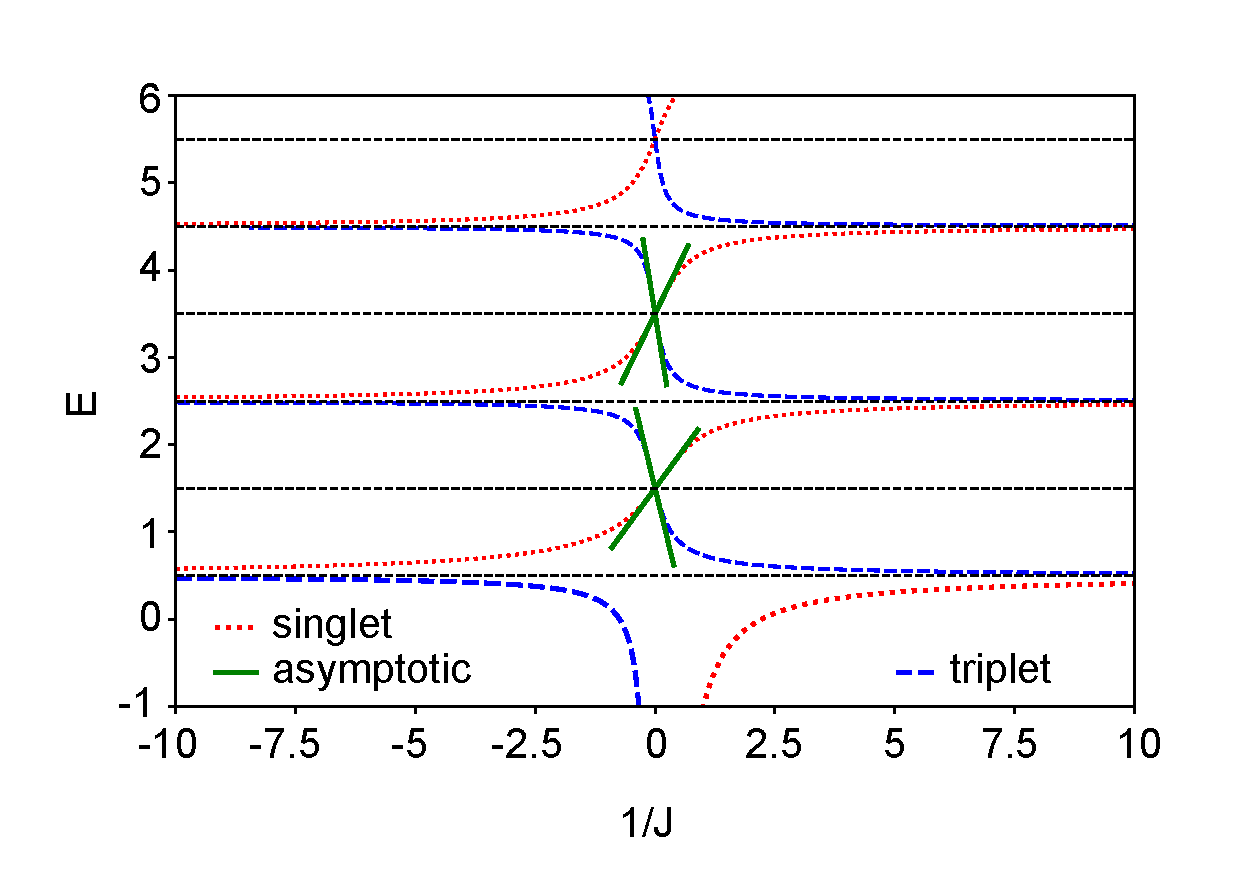
\includegraphics[width=0.7\textwidth]{fig1.pdf}
    \bicaption{一个杂质与一个费米子的1+1体系在$S_{tot,z}=0$子希尔伯特空间的能谱随自旋交换相互作用强度的变化。蓝色虚线(红色散点线)代表自旋三重态(自旋单重态)通道中的本征解。绿色实线代表强相互作用附近的微扰论渐近行为。其横纵坐标$E$与$J$的量纲为$\omega$与$\sqrt{\omega/M}$。}{(Color online). Energy spectrum of one fermion and one impurity in $S_{tot,z}=0$ subspace. The blue dashed (red dotted) lines show $E_t$ ($E_s$) for spin-triplet (singlet) eigen-states. The green solid line shows the asymptotic fitting to (\ref{asymptotic}) in strong coupling limit. Here the units of $E$ and $J$ are respectively $\omega$ and $\sqrt{\omega/M}$.}
    \label{fig:fig1}
\end{figure}

首先对于自旋单重态通道的解,对角化后的自旋交换相互作用对应强度为$\gamma_s=-3J/2$的接触相互作用,因此只有在$J>0$的时候,在散射态临界下面会有束缚态的产生。正如图~\ref{fig:fig1}~最下面的红色散点线所示,我们从$J=0$逐渐增大到$J=+\infty$,自旋单重束缚态的能量越来越低,在$J\to + \infty$附近,$E_s$渐近行为为$E_s\rightarrow -9J^2/8$。我们称这样的态为lower attractive branch。除了这支束缚态以外,我们发现其余的本征态在$J\to \pm \infty$的时候都趋近于有限大小的谐振子奇数能级,远远位于束缚态之上,我们称这样的一系列态为repulsive upper branch。如果我们逐渐放松谐振子的束缚程度,取$\omega\to 0$,我们会发现lower branch将变为一维接触势的唯一束缚态,而upper branch将变为一系列散射态。

对于自旋三重态通道的解,对角化后的自旋交换相互作用强度为$\gamma_t=J/2$,因此只有在$J<0$的时候才存在束缚态,如图~\ref{fig:fig1}~中最下面的蓝色虚线所示,当我们从$J=0$往负方向调节$J\to-\infty$时候,束缚态的能量不断降低,在$J\sim -\infty$附近其渐近行为是$E_t\rightarrow -J^2/8$。我们称这种态为lower attractive branch。类似地,在束缚态的上面,有一系列repulsive upper branch,它们的能量随$J\to-\infty$而趋近于谐振子的奇数能级处。

在$1/J=0$附近,我们看到不论单重态还是三重态的repulsive upper branch 能量都具有很好的线性行为,这表明此处可用微扰论来描述。具体地,我们假设渐近行为是:



\section{小结与展望}\label{sec:spex-summary}

